\ifx\wholebook\relax \else

\documentclass[b5paper]{article}
\usepackage[nomarginpar
  %, margin=.5in
]{geometry}

\addtolength{\oddsidemargin}{-0.05in}
\addtolength{\evensidemargin}{-0.05in}
\addtolength{\textwidth}{0.1in}

\usepackage[en]{../prelude}

\setcounter{page}{1}

\begin{document}

\title{Zero}

\author{Xinyu LIU
\thanks{{\bfseries Xinyu LIU} \newline
  Email: liuxinyu99@hotmail.com \newline}
  }

\maketitle
\fi

\markboth{Zero}{A tour of numbers}

\ifx\wholebook\relax
\chapter{Zero}
\fi

\epigraph{The truth of Being and of Nothing is accordingly the unity of the two: and this unity is Becoming.}{Hegel {\em Short Logic}}

Despite the history of number is over 5000 years, the history of zero is only about 1200 years. Zero is a new comer. It was originated from India, and was introduced to the west through Arabian. Different from 1, 2, 3, ... zero was created as a placeholder but not a number. It looked like a second level citizen in the kingdom of numbers because zero has no value.

\section{Rejection of zero}
People created zero to express nothing. Indian named it as sunya, which meant vacant in Sanskirt. For example, the 0 in number 2025 means there is {\em no} value of hundred. 0 indicates void, which gives negative meaning in the tradition of west (cultural, philosophical, and religious). It was connected with darkness, ending, and death. While 1 means being, there is a thing; 2 means there are two things... One says there is no apple, but not say there is zero apple. In such way, it emphasizes the negate of being. Shakespeare wrote `To be or not to be, that is the question.'

\index{Roman abacus}
\begin{figure}[htbp]
 \centering
 \includegraphics[scale=0.35]{img/Roman-abacus}
 \caption{A bronze Roman abacus in 1st century. There are counting beads in the grooves; each groove represents Roman unit I, V, X, C, and M\cite{Cartwright-2013} (Archaeological Museum, Aosta, Italy).}
 \label{fig:roman-abacus}
\end{figure}

Although seen the big advantage of Hindu-Arabic numeral system in computation, the European people converted the result to Roman numbers in order to avoid zero\footnote{Similarly, Chinese people left empty positions for zero when computing with the counting rods (see \cref{sec:counting-rods}), but they converted the result to the number in multiplicative grouping system, such as a hundred, two thousand and fifteen, a hundred and two. The dedicated character of zero `零' didn't appear until Song and Yuan dynasty.}. Some people treated 0 evil and only used it privately. Clergies computed in Roman numbers with abacus shown in \cref{fig:roman-abacus} (not the Chinese abacus). This tool is derived from Babylonian tablet. The method is to move/change beads among grooves, then record the result in Roman numbers. As more and more people, particularly merchants and bankers, adopted Hindu-Arabic numerals in practice, a challenge between the two systems happened in the 16th century (as in \cref{fig:hindu-arabic-vs-abacus}). It's not hard to imagine the result, Hindu-Arabic system won. Such challenges repeated several times in the history: Stephenson's Rocket, a pioneering steam-powered locomotive vs. horse\footnote{Invented by British engineers George and Robert Stephenson.} in 1830; IBM Deep blue vs. the world chess champion Garry Kasparov in 1997; Google's Alpha-Go vs. 9-dan Go master Lee Sedol and Ke Jie; Open AI's ChatGPT vs. students in SAT test... Every time a revolutionary thing arising, a challenge happens.

\begin{figure}[htbp]
 \centering
 \includegraphics[scale=0.8]{img/Hindu-arabic-vs-abacus}
 \caption{Engraving of Arithmetica (or the Allegory of Arithmetic) supervising a contest between Boethius, representing written calculation using Hindu-Arabic numbers, and Pythagoras, represented as using a counting board. From Gregor Reisch, {\em Margarita philosophica} in 1503.}
 \label{fig:hindu-arabic-vs-abacus}
 %https://old.maa.org/press/periodicals/convergence/mathematical-treasures-margarita-philosophica-of-gregor-reisch
\end{figure}

The win of Hindu-Arabic system gave 0 `citizenship', legitimate to use. But it's a second class citizen. Why 0 can't be first class citizen as $1, 2, 3, \dotsc$?

\section{To be a number}

What does make 0 different from $1, 2, 3, \dotsc$ preventing it from being a first class citizen? It's the value, or magnitude. The value of 1 is 1, for example, the length of 1cm, the mass of 1 gram, the unit of 1 sheep... the value of 2 represents the length of 2cm, the mass of 2 grams, the units of 2 sheep... But what's the value of 0? It has no value. 0 is a placeholder, but not a number because it has no value\cite{Seife-2000}. 0 is so different that it breaks those rules work well for $1, 2, 3, \dotsc$ for example:

\label{sec:archimedes-axiom}
\begin{enumerate}[1)]
\item Archimedes axiom. A number\footnote{All numbers refer to natural number in this section.} increases when adding to itself. Archimedes treated it as an axiom: for any non-zero $m < n$, there is a time that $m + m + \cdots > n$. \index{Archimedes axiom}

\begin{align*}
1 + 1 &= 2   & 1 + 1 + 1 &= 3 & \dots \\
2 + 2 &= 4   & 2 + 2 + 2 &= 6 & \dots \\
3 + 3 &= 6   & 3 + 3 + 3 &= 9 & \dots \\
\dots &      & \dots     &    &
\end{align*}

But $0 + 0 = 0$ does not increase, $0 + 0 + 0 + \cdots$ will never exceeds any number, such as 1.

\item Product. People recognized product from arranges pebbles (or soldiers) in rectangle. $1 \times 5 = 5$ is a rectangle of 1 row and 5 columns; $2 \times 5 = 10$ is a rectangle of 2 rows and 5 columns; $3 \times 5 = 15$ is a rectangle of 3 rows and 5 columns... but what is $0 \times 5$ for? the rectangle vanishes as shown in \cref{fig:grid-vanish}.

\begin{figure}[htbp]
 \centering
   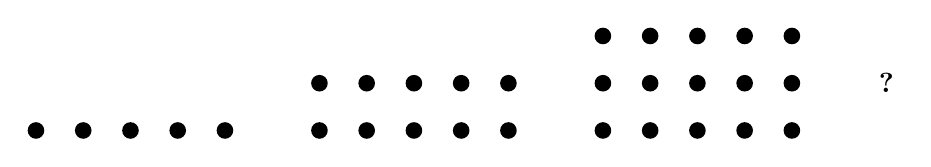
\begin{tikzpicture}[
       scale=0.6,
       dot/.style={circle, fill=black, minimum size=6pt, inner sep=0pt},
       question/.style={font=\Huge, font=\bfseries}
   ]

   \foreach \x in {0,1,2,3,4} {
       \node[dot] at (\x, 0) {};
   }

   \foreach \x in {0,1,2,3,4} {
       \foreach \y in {0,1} {
           \node[dot] at (\x + 6, \y) {};
       }
   }

   \foreach \x in {0,1,2,3,4} {
       \foreach \y in {0,1,2} {
           \node[dot] at (\x + 12, \y) {};
       }
   }

   \node[question] at (18, 1) {?};
   \end{tikzpicture}

 \caption{The rectangle vanishes for $0 \times 5$.}
 \label{fig:grid-vanish}
\end{figure}

\label{sec:mul-as-zoom}
Multiplication means scaling. When scale a ruler 2 times, not only the length of the ruler, but also the length between marks double; when scale 3 times, both the length of the ruler and between marks triple, as shown in \cref{fig:ruler-vanish}. If scale down to $\frac{1}{3}$, then we get a small ruler. But what if scale 0 (times 0)? The ruler together with the marks collapses to a dot; it vanishes.

\begin{figure}[htbp]
 \centering
 \includegraphics[scale=0.35]{img/zoom-rulers}
 \caption{The ruler with marks collapses to a dot without size when scaling 0.}
 \label{fig:ruler-vanish}
\end{figure}

The product represents rectangle; the ruler represents line segment. Multiplication by 0 destroys them. There was no zero in Greek geometry or numeral system. Euclid defined `a point is that which has no parts; a line is length without breadth.' (Definition 1 and 2 in Book I of {\em Elements}.) Is 0 a point?

\item Division is the reverse of multiplication. For example, the reverse of $2 \times 3 = 6$ is $6 \div 2 = 3$; the reverse of $3 \times 4 = 12$ is $12 \div 3 = 4, \dotsc$ the reverse of $2 \times 0 = 0$ is $0 \div 2 = 0$, generally the reverse of $a \times 0 = 0$ is $0 \div a = 0$. However, what would be division by 0?From the reverse of multiplication, $a \div b$ is to find some $c$ satisfying $bc = a$; it means $a \div 0$ is to find some $x$ satisfying $0x = a$. But $0x = 0$, unless $a \ne 0$, there isn't such a $x$, because $0x = 0 \ne a$. Even if $a = 0$ such that the reverse of $0 \times 0 = 0$ looks like $0 \div 0 = 0$, but then the reverse of $1 \times 0 = 0$ will be $0 \div 0 = 1$; the reverse of $2 \times 0 = 0$ will be $0 \div 0 = 2, \dotsc$ any reverse of $a \times 0 = 0$ will be $0 \div 0 = a$, hence $0 \div 0$ can be any number, that is$(0 \div 0) = 0 = 1 = 2 = 3 = \cdots$ Nothing, which is 0, would become being like $1, 2, 3, \dotsc$ Bertrand Russell, in a lecture on logic, mentioned that in the sense of material implication, a false proposition implies any proposition. A student raised his hand and said ``In that case, given that 1 = 0, prove that you are the Pope.'' Russell immediately replied, ``Add 1 to both sides of the equation: then we have 2 = 1. The set containing just me and the Pope has 2 members. But 2 = 1, so it has only 1 member; therefore, I am the Pope.'' \index{0!division by zero}

\begin{align*}
0 = 1 & \Rightarrow 1 = 2     & \text{add 1 to both sides} \\
      & \Rightarrow 1 + 1 = 3 & \text{add 1 to both sides} \\
      & \dotso
\end{align*}

Ian Stewart gives another ridiculous example\cite{Stewart-2019}:

One cat has one tail;

Zero cat has eight tails.

Therefore, adding: One cat has nine tails.
\end{enumerate}

As 0 breaks rules exceptionally, people treat 0 different from $1, 2, 3, \dotsc$. As shown in \cref{fig:keyboard}, 0 comes after numbers 1 to 9.

\begin{figure}[htbp]
 \centering
 \includegraphics[scale=0.35]{img/keyboard}
 \caption{0 in keyboard}
 \label{fig:keyboard}
\end{figure}

\subsection{Ordinal number}
Besides value, number has order. 1 goes first, 2 follows 1, 3 follows 2, and so on. People recognize order from counting. Michael Artin had a conversation with his daughter\cite{MArtin-2011}:

``One, two, three, five, four...''

``No Daddy, it's one, two, three, four, five.''

``Well if I want to say one, two, three, five, four, why can't I?''

``That's not how it goes.''

\begin{center}
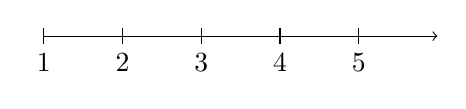
\begin{tikzpicture}
    \draw[->] (-2,0) -- (3,0); % node[right] {$x$};
    \foreach \x in {1,2,3,4,5}
    {
        \draw (\x-3,0.1) -- (\x-3,-0.1) node[below] {$\x$};
    }
    % \draw[fill=black] (-2,0) circle (0.05); % origin
\end{tikzpicture}
\end{center}

\index{数轴} \index{序数} \index{公元纪年}

Arrange numbers in a line, namely the number line. Each number has an order (its ordinality). Our dating system came from an idea of a Christian Monk Dionysius Exiguus in 525 CE. He defined the year that Jesus Christ's birth as {\em Anno Domini}, a Latin term which means Year of our Lord. It was abbreviated as AD. It changes to CE, stands for {\em Common Era} to include all religions nowadays. Because the Christmas day was December 25th, which is close to the year end, 1 CE actually started from the next January 1st. Then followed 2 CE, 3 CE... The years before that is called {\em Before Christ}, abbreviated as BC. For the same reason, we use BCE, stands for {\em Before Common Era}. More people adopt BCE/CE to replace BC/AD. The previous year of 1 CE is 1 BCE, the previous of 1 BCE and 2 BCE... Note there isn't 0 between 1 BCE and 1 CE. It causes an exceptional problem. For example, Octavian defeated rivals of Mark Antony and Cleoptra, consolidated power, and became Augustus in the year of 27 BCE, which started Roman empire; The unified empire ended with the death of Emperor Theodosius I in 359 CE. How long is Rome empire? The calculation of $27 + 359 = 386$ years actually is 1 year more than the correct answer. To make it clear, consider a baby born on December 25th, 1 BCE, how old would be on November 25th, 1 CE? Definitely not a full year of age 1, but only 11 months. The baby would be 1 year old on December 31st, 1 CE, but not $1 + 1 = 2$ years old. On the contrary, For a baby born on 1 CE, how old would be it in 2 CE? It would be $2 - 1 = 1$ year old. In general, from $x$ CE to $y$ CE, there are $y - x$ years. At 11:59:50 on December 31st, 1999, all people were counting down for the new millennium, however, from the beginning of CE, which is 1 CE to 2000 CE, there are only $2000 - 1 = 1999$ years. We celebrated 1 year earlier than a true millennium. Why does such error occur? Because we skipped 0 CE, which was missed unfortunately. If you didn't follow, consider this example: It is the second after 11:59:59 at night starts a new day. In other word, a day start at 0:00:00; the first second of a day is 0:00:01. Look at the clock plate to confirm a day starts at zero o'clock but not one o'clock.

\begin{figure}[htbp]
 \centering
 \includegraphics[scale=0.35]{img/thermometer}
 \caption{A thermometer likes a number line in vertical.}
 \label{fig:thermometer}
\end{figure}

\index{thermometer}
A thermometer, as shown in \cref{fig:thermometer}, measures temperature. 0$\degree$C (zero degree of Celsius scale) is defined as the melting point of pure water (or ice-water mixture) at standard atmosphere pressure. 100$\degree$C is defined as the boiling point of pure water at standard atmosphere. Divide the length between them of the thermometer into 100 units, 1 unit for a degree. In this way, the mark at 3 has the scale of 3$\degree$C, 4 has the scale of 4$\degree$C...$x$ has the scale of $x\degree$C. from 5$\degree$C below the freezing point to 10$\degree$C above the freezing point, there are 15 degrees. It avoids the calendar problem of BC/BCE. If turn the thermometer horizontally, we then get a number line. 0 is at the position left to $1, 2, 3, \dotsc$. In this context, 0 does not mean nothing, but the starting point, the origin.

\begin{center}
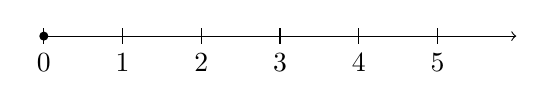
\begin{tikzpicture}
    \draw[->] (-3,0) -- (3,0); % node[right] {$x$};
    \foreach \x in {0,1,2,3,4,5}
    {
        \draw (\x-3,0.1) -- (\x-3,-0.1) node[below] {$\x$};
    }
    \draw[fill=black] (-3,0) circle (0.05); % origin
\end{tikzpicture}
\end{center}

\label{sec:zero-as-ordinal} \index{0!ordinal}
If number $a$ is on the left of number $b$, it means the order of $a$ is {\em before} $b$, or $a < b$, with distance of $b - a$; if $a$ is on the right of $b$, it means $a$ is {\em after} $b$, or $a > b$, with distance of $a - b$. We can combine this two cases by only defining $a < b$ as {\em before}, and negate it for the other. Alternatively, we may consider $a + d$ as to move $a$ forward (to the right) by $d$; $a - d$ to move backward (to the left) by $d$; if $d = 0$, then $a + 0 = a - 0 = a$, which {\em fixes} $a$. 0 has a valid order as those of 1, 2, 3, ..., but not a second class citizen.

\index{array}
Array is a data structure in computer system. It stores a collection of values in a consecutive cells in memory. For example,

\begin{lstlisting}[language=C, frame=single]
int a[10];
\end{lstlisting}

This line of code defines $a$ as an array, which stores 10 integers. Suppose an integer has 16 bits in the computer, the maximum integer is $2^{16}-1 = 65535$, which is $1111...1$ of sixteen 1s in binary; 314 is $100111010(=256 + 32 + 16 + 8 + 2)$ in binary, i.e., the bits at position 9, 6, 5, 4, 2 are 1, the other 11 positions are 0 (see \cref{sec:binary-numerals}). A byte has 8 bits, hence an integer of 16 bits occupies 2 bytes, or denoted as \lstinline|sizeof(int) = 2B = 16|. An array of 10 integers occupies $2 \times 10 = 20$ bytes in memory.

When executes the code \lstinline|int a[10]|, the computer will allocate 20 bytes in the memory\footnote{The are two types of memory: stack and heap; It is stack in this example.}, and point \lstinline|a| to the beginning position, called address. The program next uses this address to index an element of the array. The next two bytes from \lstinline|a| stores the first element; the 3rd and 4th bytes from \lstinline|a| stores the second element. The array stores 1, 2, ..., 9 as shown in \cref{fig:array}.

\begin{figure}[htbp]
 \centering
 \includegraphics[scale=0.35]{img/array}
 \caption{Array}
 \label{fig:array}
\end{figure}

Note the first element starts from \lstinline|a|. The distance between its address and \lstinline|a| is 0, denoted as \lstinline|a[0]|; The address of the next element starts from \lstinline|a + sizeof(int) = a + 16|, denoted as \lstinline|a[1]|; the next elements starts from \lstinline|a + 2 * sizeof(int)|, denoted as \footnote{`*' means multiplication}\lstinline|a[2]|... The computer indexes \lstinline|a[i]| at the position of \lstinline|a + i * sizeof(int)|. The 10 elements of the array are indexed as \lstinline|a[0], a[1], ..., a[9]|. This is the reason why array starts from 0 to $n - 1$ in programming: the index $i$ is the {\em distance} between element \lstinline|a[i]| and the starting address. Distance is from 0, the true starting point. Below example puts 1 to 10 into the array:

\begin{lstlisting}[language=C, frame=single]
int a[10];
for (int i = 0; i < 10; ++i) { a[i] = i + 1; }
\end{lstlisting}

There is a joke. A programmer treated his family to the restaurant after hard work of days and nights. He asked his kid how many meat balls in the dish. The kid pointed and counted 0, 1, 2, 3, ... Mom sighed he was born a programmer.

Many kids suffer from the `planting problems' in school. For example, (1) there are trees every 10 meters along a street of 100 meters long, how many trees in total? (2) There are trees every 20 meters around the playground of 400 meters long, how many trees in total? For problem (1), treat the street as the number line; start from 0, the 0th tree, the 1st tree, the 2nd tree, ..., the 10th tree. The distance between the $i$th tree and the starting point is $10i$ meters. As $100 \div 10 = 10$, the distance between the 10th tree and the starting point is 100 meters. 0, 1, 2, ..., 10, there are total 11 numbers, hence 11 trees. For problem (2), count from 0. As the circle (the shape of the playground) is 400 meters long, $400 \div 20 = 20$, the distance between the 20th tree and the starting point is 400 meters. The position of 20th tree overlaps with the 0th, hence is skipped. 0, 1, 2, ..., 19, $\cancel{20}$, there are total 20 trees. When shall we count from 1 and when count from 0? (see \cref{qn:count-from})

\subsection{Cardinal numbers}
\index{cardinal numbers}

It's incredible to change the view of zero from `nothingness' to `origin'. Different civilizations have diverse culture. The Genesis myth describes a state of chaos and nothingness before the world began, with heaven, earth, light, and beings marking the origin of the world. Buddhism holds the world we perceive is merely an illusion, the essence is nothingness. Ancient Chinese believed that yin and yang were the forces driving all changes, and that the vast universe emerged from the chaotic Tai Chi. With the integration of civilizations, the understanding of nothingness evolved. For example, Hegel started his logic with Being, Nothing, and Becoming (the quotation at the beginning of this chapter). According to the Big Bang theory, our universe originated from a massive explosion 13.8 billion years ago, there was no time or space prior to this event.

\index{empty set} \index{Frege}

If 0, as an ordinal number, is the starting point, can it become a cardinal number as the origin of beings? 3 as a cardinal number means there are three things, for example, 3cm: the length of 3 centimeters, 3g: the mass of 3 grams, 3 sheep, and so on; they are all three concrete things; The cardinal number 3 abstracts all collections of three things. In the language of set theory, it is a set of three elements, like $\{\bigstar, \square, \bigcirc \}$ or $\{a, b, c\}$. This is how logician Frege's definition of numbers. 0, which means nothing, is the cardinal number of the empty set (a set of nothing), denoted by $\varnothing$. This symbol was created by Bourbaki (a pen name of a group of anonymous mathematicians) in 1939. 1 is the cardinal number of a set of an element (a singleton) like $\{ \bigstar \}$, $\{ a \}$, or even $\{ \varnothing \}$. It is a set of set, containing the empty set as the only one element. The cardinal number of $\{ \varnothing \}$ is 1. As such, 1 arises from 0, nothing becomes being. We may go on constructing 2 from 1 by $\{ \varnothing, \{ \varnothing \} \}$. This set contains two distinct elements, both are sets: the empty set $\varnothing$ and $\{ \varnothing \}$. As 3 is the cardinal number of a set of three things, we then construct $\{ \varnothing, \{ \varnothing \}, \{ \varnothing, \{ \varnothing \} \}\}$, and so on.

\begin{tabular}{l|l}
  Cardinal number & set \\
  \hline
  0 & $\varnothing$ \\
  1 & $\{ \varnothing \}$ \\
  2 & $\{ \varnothing, \{ \varnothing \} \}$ \\
  3 & $\{ \varnothing, \{ \varnothing \}, \{ \varnothing, \{ \varnothing \} \}\}$ \\
  $\cdots$ & $\cdots$ \\
  $n$ & $\{ \varnothing, \{ \varnothing \}, \cdots \}$
\end{tabular}

Something is created from nothing. This table lists the steps from 0 to 1, to many.

\section{Negative numbers}
\index{negative numbers}

0 is the key to the magic box. Once is accepted, many questions arises: (1) 0 is prior to 1, what is prior to 0? (2) 1 is less than 2, 3, ... 0 is less than 1, what is less than 0? (3) What is the result of $a - b$ if $b > a$?

\index{九章算术} \index{数学家!刘徽} \index{正负术}
到1500年左右,零已被人接受作为一个数,但负数的历史比零更短。16世纪和17世纪的大多数数学家并不承认它们是数\citepage[208页]{MKlein-1972}。最早使用负数的是古代中国人。在汉代的《九章算术》中,已经有完整的“正负术”,如卷八中:“同名相除,异名相益……其异名相除,同名相益……”翻译成白话文的意思是:“(做减法时)正负相同值相减,正负相反值相加……(做加法时)正负不同值相减,正负相同值相加。”刘徽在注释中说:“今两算得失相反,要令正负以名之。正算赤,负算黑,否则以邪正为异。”翻译成白话文的意思是:“如果在计算中两个量所代表的意思相反,一个代表得到,一个代表失去,就需要用“正”、“负”来命名它们。用红色算筹表示正数,用黑色算筹表示负数(见第\ref{sec:counting-rods}节算筹部分)。如果手头没有不同颜色的算筹,就把一个正着放、一个斜着放加以区分。”\cite{Jiuzhang-2009}

可见中国古人在用算筹计算时,有两种不同颜色的算筹:红色代表正数,黑色代表负数。并形成了系统的计算规则。对正负数的实际意义也有解释,用正数表示卖出(对应收入),用负数表示买入(对应支出)。这既源于战国时代后日益繁荣的商业贸易,又源于传统思想文化中的阴阳概念。如\cref{fig:yinyang}所示,红色的阳对应正,黑色的阴对应负。直到今天,我们仍然在医疗检测时说结果是阴性、阳性\footnote{阴性的英文为negative(负),阳性的英文为postive(正)。},在电化学中说电极是阴极、阳极。

\begin{figure}[htbp]
 \centering
 \includegraphics[scale=0.1]{img/yinyang}
 \caption{阴阳}
 \label{fig:yinyang}
\end{figure}

\index{数学家!婆罗摩笈多}
古希腊文明将数的概念建立在几何之上。长度、面积、体积对应着几何图形的线段、形状、占据的空间。它们自然都是正的,没有形成负数的概念。伴随着十进制位值制系统和零的演进,印度数学在7世纪出现了负数。数学家婆罗摩笈多(公元589~670年,见\cref{fig:Brahmagupta})在他的著作中明确地区分正负数。他用财富和负债赋予正负数实际意义,使用特殊的符号标记负数,并给出了一系列的规则,如\cite{Rogers-2011}:

\begin{multicols}{2}
\begin{enumerate}[1)]
\item 债务减零是债务。
\item 财富减零是财富。
\item 零减零为零。
\item 零减负债是财富。
\item 零减财富是负债。
\item 零乘以负债或财富是零。
\item 零乘以零为零。
\item 财富与财富的积或商是财富。
\item 负债与负债的积或商是财富。
\item 财富与负债的积或商是负债。
\item 负债与财富的积或商是负债。
\end{enumerate}
\end{multicols}

\begin{figure}[htbp]
 \centering
 \includegraphics[scale=0.3]{img/Brahmagupta}
 \caption{婆罗摩笈多(安德里亚斯・施特里克绘)}
 \label{fig:Brahmagupta}
\end{figure}

\index{数学家!丢番图}
古希腊亚历山大时代的数学家丢番图(公元200~284年)开始独立于几何之外研究算术问题。他使用符号代表未知量,考虑了一次方程和二次方程的解。在他的著作《丢番图算术》中有一道题目:求方程$4 = 4x + 20$的解。面对引出的负数解,丢番图认为它是荒谬的。公元9世纪,阿拉伯数学家从印度的数学和天文学著作中接触到了负数,但他们同时又受到古希腊数学的影响,从而对负数产生了矛盾的态度。数学家花拉子密一方面接受负数的概念及其运算规则,并将其应用到解方程的移项与对消中,但另一方面,他使用几何论证方法的正确性,因此不得不排斥负数。花拉子密不能像我们今天一样用$ax + b = 0$概括所有一次方程,也不能能用$ax^2 + bx + c = 0$概括所有二次方程。为了避免负系数,他把方程划分为6类,如$ax = b$、$b - ax = 0$、$ax^2 + bx = c$、$bx + c = ax^2$、$ax^2 + c = bx$等。直到15世纪,欧洲学者才开始接触、研究负数。16世纪,意大利数学家卡尔达诺\footnote{也有人译作卡尔丹}(1501~1576年)在他的著作《大数》\footnote{拉丁文名为Ars Magna,出版于1545年。}中给出了一般三次、四次方程的公式解法。他同样遵循古希腊传统,使用几何证明正确性。把一次项解释为长度、二次项解释为面积、三次项解释为体积。不接受负数作为方程的系数。卡尔达诺不得不给出了60种不同类型的方程。

\subsection{序数}
\index{数学家!沃利斯} \index{数轴} \index{负序数}
17世纪,英国数学家沃利斯(1616~1703年)引入了数轴,并通过序数理解负数的意义。从序数上说,负数是0之前的部分,我们看下面两个例子。

\begin{example}
公元纪年。以耶稣基督诞生的一年为公元1年,此后为公元2年、3年……那么在耶稣诞生前呢?依然有时间,有历史事件发生。这些历史事件发生在公元前。耶稣诞生前的年份依次是公元前1年、公元前2年……公元前的年份蕴含着负数的意义(注意,这里缺少公元0年)。
\end{example}

\begin{example}
温度。进入冬天,气温逐渐下降,终于3度、2度、1度、0度,降到了冰点。但0度不是终结,尽管水凝固成冰,但随着温度继续下降,温度计上的红色煤油液面跨过了0度,降到了零下1度、零下2度……零下的温度比0度低,它们是负温度。
\end{example}

把温度计横过来,并向两边无限延伸,我们就得到了数轴:

\begin{center}
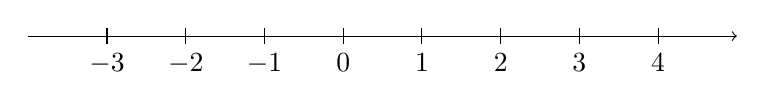
\begin{tikzpicture}
    \draw[->] (-4,0) -- (5,0);
    \foreach \x in {-3,-2,-1,0,1,2,3,4}
    {
        \draw (\x,0.1) -- (\x,-0.1) node[below] {$\x$};
    }
\end{tikzpicture}
\end{center}

负数作为序数在0和任何正数的左侧。0分开了正数、负数,位于中间。我们在第\ref{sec:zero-as-ordinal}介绍的规则依然成立:若$a < b$,$a$在$b$的左边,如果$b = 0$,$a$为负数,如果$a = 0$则$b$为正数。在序数意义下,小于“$<$”和大于“$>$”关系还可以用差的正负来表示。$a - b < 0$则$a < b$,$a$在$b$的左边\footnote{$a < b$,两边减$b$:$a - b < b - b = 0$}。$a - b > 0$则$a > b$,$a$在$b$的右边。若$d > 0$则$a + d$向前(右)移动$d$,$a - d$向后(左)移动$d$,若$a < d$,则移动到负数的区域。如果$d < 0$则移动的方向相反:$a + d$向后(左),$a - d$向前(右)。

\subsection{基数}
\index{负号}
尽管沃利斯用数轴给出了负数的意义,但他却奇怪地认为负数比无穷大,但不小于零。在《无穷大的算术》\footnote{拉丁文名为Arithmetica Infinitorum,1655年出版}中,沃利斯写到:由于比例$a/0$在$a$为正数时是无穷大\footnote{沃利斯是微积分的早期先驱之一,当时尚未形成严密的极限概念。若$a$、$b$都是正数,当观察到随着$b$减小到接近0时,$a/b$变得很大,于是随意地认为$a/0$是无穷大。},故当分母变为负数时,例如当$a/b$中的$b$是负数时,这个比必定大于无穷大\cite{MKlein-1972}。这都说明人们对于负数作为基数的意义感到困惑。总体来说,16世纪和17世纪,并没有很多数学家对于使用负数心安理得或者承认它是数,更谈不上承认它们可以作为方程的真实的根\cite{MKlein-1972}。笛卡尔的坐标系只有第一象限,帕斯卡则认为从0减去4纯粹是胡说。天文学家第谷·布拉赫使用了符号“-”来标识负数,但他认为负数只能私下使用。
%% https://web.ma.utexas.edu/users/mks/326K/Negnos.html

\index{绝对值}
负数引起的困惑是可以理解的。以温度为例,零下三十几度的南极洲显然比零下二十几度的东北地区更寒冷。从寒冷的程度看,如果基数表现大小,似乎南极洲温度的基数更大,但从数轴上的序数看$-30 < -20$。从年代上看,孔子(公元前551~公元前479年)生活的时代比孟子(公元前372~公元前289年)生活的时代更久远。如果基数表现大小,似乎孔子时代年份的基数更大,但从纪年的序数看$-479 < -372$。这些问题逐渐使我们认识到\underdot{绝对值}的概念。在数轴上,一个数$a$的绝对值是$a$到0的距离(长度),例如正数5的绝对值是$5 - 0 = 5$,即5本身;负数$-5$的绝对值是$0 - (-5) = 5$。在数轴上-5和5关于0对称,彼此称为对方的相反数。$a$的相反数是$-a$。而0到自己的距离是0 - 0 = 0。这样归纳下来,数轴上一个数$a$的绝对值记作$|a|$,有3种情况:

\[
|a| = \begin{cases}
  a & a > 0 \\
  0 & a = 0 \\
  -a & a < 0
\end{cases}
\]

\index{数学家!范·德·瓦尔登} \index{数偶} \label{sec:z-as-pair}
用语言描述就是,正数和零的绝对值是它本身,负数的绝对值是它的相反数。二十世纪初,范·德·瓦尔登在《代数学》\footnote{原名《近世代数》。数学家范·德·瓦尔登当时从荷兰来到德国哥廷根求学,他根据埃米尔·阿廷和艾米·诺特的演讲和讨论班内容整理出了这本抽象代数讲义,影响了一代数学家。}一书中给出了一个“构造”负数的方法\citepage[8页]{van-der-Waerden-2009}。用一对数偶$(a, b)$来表示整数如下:
\begin{itemize}
\item 用$(a + b, b)$表示自然数$a$。
\item 用$(b, b)$表示0。
\item 用$(b, a + b)$表示负数$-a$。
\end{itemize}

例如(3, 1)表示2, (5, 5)表示0,(100, 101)表示-1。我们可以把$(a, b)$想象成天平两边的质量,天平平衡时$(b, b)$两边质量相等,左右的的质量差为0;天平左侧质量更大的时候,左右质量差为正数;天平右侧质量更大的时候,左右质量差为负数。每个数都有许多表示,例如$(3, 1) = (9, 7) = (360, 358) = \cdots$都表示2;$(5, 5) = (100, 100) = (128, 128) = \cdots$都表示0;$(100, 101) = (1, 2) = (8, 9) = \cdots$都表示$-1$。但每个符号$(a, b)$定义一个,且只定义一个整数,即:

\begin{itemize}
\item 用$a > b$表示自然数$a - b$。
\item 用$a = b$表示0。
\item 用$a < b$表示负数$-(b - a)$。
\end{itemize}

接下来为数偶定义加法和乘法:

\begin{align}
(a, b) + (c, d) &= (a + c, b + d) \\
(a, b) \cdot (c, d) &= (ac + bd, ad + bc)
\label{eq:pair-add-mul}
\end{align}

例如加法$2 + (-1) = (5, 3) + (2, 3) = (7, 6) = 1$,乘法$-2 \times 3 = (1, 3) \cdot (5, 2) = (1 \times 5 + 3 \times 2, 1 \times 2 + 3 \times 5) = (11, 17) = -6$。\cref{qn:pair-arithmetic}要求读者验证加法、乘法的交换律、结合律、分配律(合称五大定律)对数偶都适用。

这个方法完全不使用零和负数,只用1、2、3……形式化地定义出了正数、零、负数,绕开了历史上引起争议的问题。不禁令人想起克罗内克的话:“上帝创造了自然数,其余都是人的工作。”

\section{数轴}
引入零和负数后,数轴上就标记出了向两侧无限延伸的整数。

\begin{center}
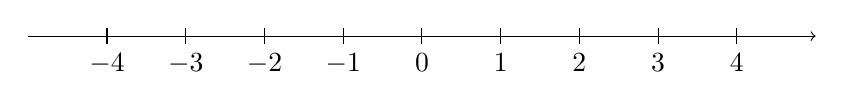
\begin{tikzpicture}
    \draw[->] (-5,0) -- (5,0);
    \foreach \x in {-4,-3,-2,-1,0,1,2,3,4}{
        \draw (\x,0.1) -- (\x,-0.1) node[below] {$\x$};
    }
\end{tikzpicture}
\end{center}

我们介绍一下标准符号的由来。0、1、2、3……叫做自然数,记作$\mathbb{N}$。是英文natural numbers的首字母。在没有认识到0以前,自然数不包括0,只有1、2、3……但随着0的引入,我们认识到0才是真正“自然”的起点、原点(见第\ref{sec:peano-axioms}节皮亚诺公理)。今天大多数定义(包括我国的部编义务教育数学教材)都把0算作自然数。通常用小写字母$n$表示某个自然数。引入负数后,负整数、零、正整数,即……$-3$、$-2$、$-1$、0、1、2、3……合称整数,记作$\mathbb{Z}$。它来自德语“数”Zahlen的首字母。正整数有时记作$\mathbb{Z}^+$,负整数记作$\mathbb{Z}^-$。整数的英文是integral number或integer,我们有时也用其首字母$i$表示某个整数。在枚举一些列的事物时,通常用$i$作下标,例如:$a_1, a_2, ..., a_i, ..., a_n$,其中$a_i$表示第$i$个。但这里的$i$不是integer,而是索引的英文index的首字母。$a_n$通常指最后一个,即第$n$个。数学家们非常重视符号的使用。好的符号形象、生动、易于理解,表达能力强,甚至具有意想不到的力量(如莱布尼茨的微积分符号)。韦达、笛卡尔开创了代数符号的传统,他们用$a, b, c$表示已知量,用$x, y, z$表示未知量。这些习惯影响至今。

\index{数轴!四则运算}
利用数轴,我们可以给出四则运算($+, -, \times, \div$)的直观解释(第3章会给出几何解释)。在\ref{sec:zero-as-ordinal}节,我们说加减$a \pm b$将数轴上的数$a$移动$b$个单位,共有五种移动情况:

\begin{center}
  \begin{tabular}{c|c|c|c}
          & $b > 0$ & $b < 0$ & $b = 0$ \\
  \hline
  $a + b$ & 向右     & 向左    & \multirow{2}{*}{不动} \\
  \cline{1-3}
  $a - b$ & 向左     & 向右
  \end{tabular}
\end{center}

我们看到$b < 0$时$a + b$相当于减法,而$a - b$相当于$a$加上$-b$。$b$和$-b$互为相反数,这样减法无非是加法的一种情况。我们可以用加法概括减法:

\begin{center}
\begin{tabular}{c|c|c|c}
        & $b > 0$ & $b < 0$ & $b = 0$ \\
\hline
$a + b$ & 向右     & 向左    & 不动
\end{tabular}
\end{center}

\begin{figure}[htbp]
 \centering
 \includegraphics[scale=0.45]{img/translate}
\end{figure}

任给数轴上两个数$a, b$,它们的距离是:

\begin{center}
  \begin{tabular}{c|c|c|c}
      & $a < b$ & $a > b$ & $a = b$ \\
  \hline
  距离 & $b - a$ & $a - b$ & $0$
  \end{tabular}
\end{center}

\begin{figure}[htbp]
 \centering
 \includegraphics[scale=0.4]{img/distance}
\end{figure}

这恰是绝对值的概念,距离等于$|a - b|$。特殊情况下,若$b = 0$,一个数$a$到原点0的距离是$|a|$。

\begin{figure}[htbp]
 \centering
 \includegraphics[scale=0.4]{img/abs}
\end{figure}

如果我们把“差”理解为“差距”,可正可负。在数轴上给定一个数$a$,它与另一个数$b$的差(距)就是$a - b$。若$a - b > 0$则$a > b$,$a$在$b$的右侧;若$a - b < 0$则$a < b$,$a$在$b$的左侧;若$a - b = 0$则$a = b$,$a$和$b$重合。特别地,$a$到原点0的差(距)$a - 0 = a$,就是它本身。

在数轴上,一个数$a$的相反数就是它关于原点0的对称点$-a$;0的相反数是它自己。

\begin{center}
\begin{tikzpicture}
    \draw[->] (-3,0) -- (3,0);
    \draw (-2,0.1) -- (-2,-0.1) node [below] {$-a$};
    \draw (2,0.1) -- (2,-0.1)   node [below] {$a$};
    \draw (0,0.1) -- (0,-0.1)   node [below] {$0$};
\end{tikzpicture}
\end{center}

0能“无中生有”:$0 \begin{cases} n \\ -n \end{cases}$,“分裂”成任何数$n$和它的相反数$-n$。反之,$n$和$-n$遇到一起“湮灭”为0,如同一对正负电荷。以上我们固定数轴,移动数轴上的数(点)。运动是相对的,我们也可以移动变换整条数轴:

\subsection{平移}
\index{数轴!平移}
把数轴上的\underdot{所有}数$+1$相当于把整条数轴怎样移动呢?向右?请看\cref{fig:plus-1-numline}:

\begin{figure}[htbp]
  \centering
  \begin{tikzpicture}{
      \draw[->] (-3,0) -- (4,0);
      \foreach \x in {-2,-1,0,1,2,3}{
          \draw (\x,0.1) -- (\x,-0.1) node[below] {$\x$};
      }
      \draw[fill=black] (0,0) circle (0.05); % origin

      \pgfmathsetmacro{\k}{-2}
      \draw[->] (-3,0+\k) -- (4,0+\k);
      \foreach \x in {-2,-1,0,1,2,3}{
          \pgfmathtruncatemacro{\y}{\x+1}
          \draw (\x,0.1+\k) -- (\x,-0.1+\k) node[below] {$\y$};
      }
      \draw[fill=black] (0-1,0+\k) circle (0.05); % origin
      \draw[->, decorate, decoration={snake, amplitude=.4mm, segment length=2mm, post length=1mm}]
        (0,0-0.8) -- (0,0+\k+0.3) node[above right] {$+1$};
  }
  \end{tikzpicture}
  \caption{将数轴上每个数$+1$}
  \label{fig:plus-1-numline}
\end{figure}

奇怪,竟然向左移动了1格。$\{\cdots -2, -1, 0, 1, 2 \cdots \}$各自加1后变成了$\{\cdots -1, 0, 1, 2, 3 \cdots \}$,的确向左移动了1个单位。那么$-1$一定是反向,也就是向右移动了,如\cref{fig:minus-1-numline}所示。

\begin{figure}[htbp]
  \centering
  \begin{tikzpicture}{
      \draw[->] (-3,0) -- (4,0);
      \foreach \x in {-2,-1,0,1,2,3}{
          \draw (\x,0.1) -- (\x,-0.1) node[below] {$\x$};
      }
      \draw[fill=black] (0,0) circle (0.05); % origin

      \pgfmathsetmacro{\k}{-2}
      \draw[->] (-3,0+\k) -- (4,0+\k);
      \foreach \x in {-2,-1,0,1,2,3}{
          \pgfmathtruncatemacro{\y}{\x-1}
          \draw (\x,0.1+\k) -- (\x,-0.1+\k) node[below] {$\y$};
      }
      \draw[fill=black] (0-1,0+\k) circle (0.05); % origin
      \draw[->, decorate, decoration={snake, amplitude=.4mm, segment length=2mm, post length=1mm}]
        (0,0-0.8) -- (0,0+\k+0.3) node[above right] {$-1$};
  }
  \end{tikzpicture}
  \caption{将数轴上每个数$-1$}
  \label{fig:minus-1-numline}
\end{figure}

一般地,$+a$将数轴移动$-a$,$-a$将数轴移动$a$。

\begin{center}
  \begin{tabular}{c|c|c|c}
                   & $a > 0$ & $a < 0$ & $a = 0$ \\
  \hline
  $\mathbb{Z} + a$ & 向左     & 向右    & \multirow{2}{*}{不动} \\
  \cline{1-3}
  $\mathbb{Z} - a$ & 向右     & 向左
  \end{tabular}
\end{center}

这是为什么呢?记原数轴为$A$,移动后的数轴为$A'$。$A$上的每个数$x \rightsquigarrow x + a$,变成了$x' = x + a$,$A$上的$-a \rightsquigarrow -a + a = 0$,变成了$A'$上的原点。所以$A'$上的原点\underdot{对应}着原数轴上的$-a$。若$a > 0$,自然新原点(对应$-a$)在老原点(对应0)的左边,如\cref{fig:translate-number-line}所示。

\begin{figure}[htpb]
  \centering
  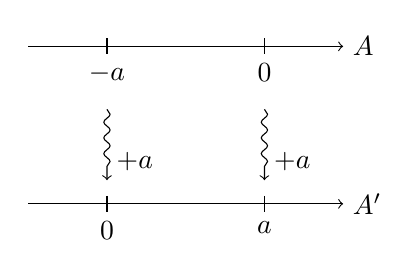
\begin{tikzpicture}{
      \draw[->] (-3,0) -- (1,0) node[right] {$A$};
      \draw (-2,0.1) -- (-2,-0.1) node[below] {$-a$};
      \draw (0, 0.1) -- (0, -0.1) node[below] {$0$};

      \pgfmathsetmacro{\k}{-2}
      \draw[->] (-3,0+\k) -- (1,0+\k) node[right] {$A'$};
      \draw (-2,0.1+\k) -- (-2,-0.1+\k) node[below] {$0$};
      \draw (0, 0.1+\k) -- (0, -0.1+\k) node[below] {$a$};

      \draw[->, decorate, decoration={snake, amplitude=.4mm, segment length=2mm, post length=1mm}]
          (-2,0-0.8) -- (-2,0+\k+0.3) node[above right] {$+a$};
      \draw[->, decorate, decoration={snake, amplitude=.4mm, segment length=2mm, post length=1mm}]
          (0,0-0.8) -- (0,0+\k+0.3) node[above right] {$+a$};
}
  \end{tikzpicture}
  \caption{数轴平移}
  \label{fig:translate-number-line}
\end{figure}

\subsection{相反数}
\index{相反数} \index{数轴!反向}
把数轴上的所有数取相反数(简称取反,英文negate)相当于把数轴反向(绕原点旋转$180\degree$)。

\begin{figure}[htpb]
  \centering
  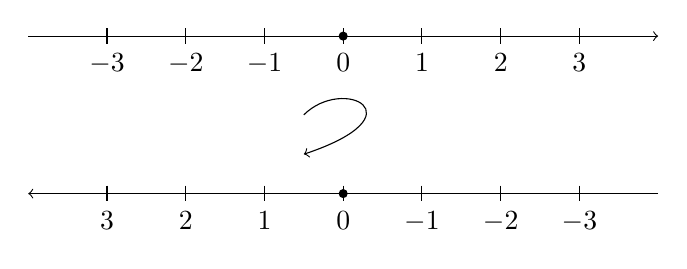
\begin{tikzpicture}{
      \draw[->] (-4,0) -- (4,0);
      \foreach \x in {-3,-2,-1,0,1,2,3}{
          \draw (\x,0.1) -- (\x,-0.1) node[below] {$\x$};
      }
      \draw[fill=black] (0,0) circle (0.05); % origin

      \pgfmathsetmacro{\k}{-2}
      \draw[->] (4,0+\k) -- (-4,0+\k);
      \foreach \x in {-3,-2,-1,0,1,2,3}{
          \pgfmathtruncatemacro{\y}{-\x}
          \draw (\x,0.1+\k) -- (\x,-0.1+\k) node[below] {$\y$};
      }
      \draw[fill=black] (0,0+\k) circle (0.05); % origin
      \draw[->] (-0.5, -1) .. controls (0, -0.5) and (1, -1.0) .. (-0.5, -1.5);
  }
  \end{tikzpicture}
  \caption{数轴反转}
  \label{fig:negate-number-line}
\end{figure}

取两次反自然会复原,即旋转$180\degree$再旋转$180\degree$等效于旋转$360\degree$,等效于不动。

\btab{ccccc}
  $\rightarrow$ & 反向 & $\leftarrow$ & 反向 & $\rightarrow$ \\
\hline
  $a$           & 相反数 & $-a$       & 相反数 & $-(-a) = a$
\etab

取相反数$a \rightsquigarrow -a$等效于乘以$-1$,即$-a = a (-1) = (-1) a$,两次取反复原就解释了“负负为正”:$-(-a) = (-1)(-a) = a$。

\subsection{缩放}
\index{数轴!缩放}
第\ref{sec:mul-as-zoom}节说乘除相当于缩放。$\times 2$把数轴放大2倍,$\times 3$把数轴放大3倍,$\div 2$把数轴缩小到$\frac{1}{2}$,$\div 3$缩小到$\frac{1}{3}$。除法是乘法的逆运算,所以$\div 2$也可以认为是$\times \frac{1}{2}$,即缩放到$\frac{1}{2}$倍,$\div 3$即缩放到$\frac{1}{3}$。这样乘除法就统一成乘法一种情况:

\begin{center}
  \begin{tabular}{c|c|c|c}
             & $a > 1$ & $0 < a < 1$ & $a = 1$ \\
  \hline
  $\times a$ & 放大     & 缩小    & 不变 \\
  \end{tabular}
\end{center}

引入负数后,如上节所说,$\times (-1)$相当于取相反数,数轴反向。$\times (-2)$相当于放大2倍后反转数轴,即$(-1) \times 2$,当然也等效于先反转数轴再放大2倍,即$2 \times (-1) = (-1) \times 2$。同样$\times (-3)$相当于放大3倍后反向,或反向后放大3倍。这样乘除法可以归纳如下:

\begin{center}
  \begin{tabular}{c|c|c|c|c|c|c}
             & $a > 1$ & $a = 1$ & $0 < a < 1$  & $-1 < a < 0$ & $a = -1$ & $a < -1$ \\
  \hline
  $\times a$ & 放大     & 不变    & 缩小          & 缩小 + 反向 & 反向 & 放大 + 反向
  \end{tabular}
\end{center}

有一种特殊情况:$\times 0$数轴“坍缩”成一点。上述“动作”可以组合:先平移$a$再平移$b$,当然这等效于先平移$b$再平移$a$,即$a + b = b + a$,这说明了加法的交换律。同样,先缩放$a$倍,再缩放$b$倍和先缩放$b$倍,再缩放$a$倍等效,即$ab = ba$,这说明了乘法交换率。我们把结合率的数轴意义作为\cref{qn:assiciative-numline}。

更复杂的组合,如先平移再缩放或反向,如$x \rightsquigarrow ax + b$,即先缩放$a$倍,再平移$-b$。\cref{qn:transform-numline}要求读者考虑如何先平移再缩放。

\section{单位元}
\index{单位元} \label{sec:unit}
0和负数成了1、2、3……一样的一等公民。它们有序数(再数轴上合法、确定的位置),有基数(确定的值)。0和其它数比起来仍是如此特殊。它是起点,它是原点,它是产生万物的“无”,还有谁像它这样独特么?1站了出来要和0比一比。

\begin{align*}
  0     &             &  1 & \\
  1 + 0 & = 0 + 1 = 1  &  1 \times 0 &= 0 \times 1 = 0 \\
  2 + 0 &= 0 + 2 = 2  &  1 \times 2  &= 2 \times 1 = 2 \\
  3 + 0 &= 0 + 3 = 3  &  1 \times 3  &= 3 \times 1 = 3 \\
  \cdots &            & \cdots & \\
  a + 0 &= 0 + a = a  &  1 \times a  &= a \times 1 =  a
\end{align*}

0加上任何数都不变,而1乘以任何数(包括0)也都不变。我们看看0和1对数轴的作用:
\begin{enumerate}[1)]
\item 加法把数轴左右平移,$+a$后数轴移动$-a$个单位($a > 0$向左,$a < 0$向右),0的作用是固定数轴不动。
\item 乘法把数轴放大缩小,$\times a$则缩放$a$倍($|a| > 1$放大,$0 < |a| < 1$缩小),1的作用是固定数轴不变。
\end{enumerate}

对于0,任何一个数$a$都能找到它的“加法双胞胎”兄弟,相反数$-a$,使得$a + (-a) = 0$。对于1,任何一个数$a$也能找到它的“乘法双胞胎”兄弟,倒数$\frac{1}{a}$,使得$a \times \frac{1}{a} = 1$,不过0没有“乘法双胞胎”兄弟。读者朋友们,你们觉得0和1谁更特殊呢?

像0和1这样“鹤立鸡群”的例子比比皆是。英语中有单词、短语、句子、段落……我们把一列英语字符叫做“字符串”,如``apple''、``hello''、``to be or not to be''、`` ''(空格)。我们可以把字符串连接在一起,如:``hello'' $\doubleplus$ `` '' = ``hello '',``hello '' $\doubleplus$ ``apple'' = ``hello apple''。不包含任何字符的串叫空串``'',把空串连接到任何字符上都不变:

\[
\text{``''} \doubleplus S = S \doubleplus \text{``''} = S
\]

如``'' $\doubleplus$ ``hello'' = ``hello'' $\doubleplus$ ``'' = ``hello''。再比如集合的并。把两个集合中包含的元素不重复地放在一起组成新的集合,如$\{a, b, c\} \cup \{1, 2, 3\} = \{a, b, c, 1, 2, 3\}$,$\{a, b, c\} \cup \{c, d, e\} = \{a, b, c, d, e\}$。空集与任何集合的并都不变:

\[
\varnothing \cup S = S \cup \varnothing = S
\]

如$\varnothing \cup \{a, b, c\} = \{a, b, c\} \cup \varnothing = \{a, b, c\}$。数学上我们把0叫做加法的单位元,1叫做乘法的单位元,空串叫做字符串连接的单位元,空集叫集合并的单位元。一般地在集合(可以有限也可以无限)$M$中,如果存在一个元素$e$,在某种二元运算$\odot$下使得:

\[
  e \odot a = a \odot e = a
\]
对$M$中的所有$a$都成立,我们把$e$叫做运算$\odot$在$M$中的单位元。例如0是加法在数的集合中的单位元,1是乘法在除去0之外的数的集合中的单位元,空串是连接操作在字符串集合中的单位元,空集是并在所有\underdot{集合的集合}中的单位元。单位元和集合中的其它元素一样是一等公民,但它是特殊的、唯一的(见\cref{qn:unique-e})。

\index{逆} \index{逆元}
对集合中的元素$a$,如果存在某个元素$b$使得$a \odot b = e$,则称$b$是$a$的逆。例如$a$在加法运算下的逆就是相反数$-a$,因为$a + (-a) = 0$。非0数$a$在乘法运算下的逆是$\frac{1}{a}$,因为$a \times \frac{1}{a} = 1$。并非所有元素都有逆,例如除了空串外,所有字符串都没有连接操作的逆;除了空集外,所有集合都没有并操作的逆。有了逆,我们就可以把加减乘除四则运算简化为“二则运算”,$a - b$只不过是$a$加上$b$的逆(相反数),$a \div b$只不过是$a$乘以$b$的逆(倒数)。

\section{皮亚诺公理}
\label{sec:peano-axioms}
1889年,意大利数学家皮亚诺为自然数建立起严格的公理化系统。它使用零作为起点,在加上“数数”这个动作,定义出了自然数。这组公理一共有五条,合称皮亚诺公理。

\index{皮亚诺公理}
\begin{enumerate}[公理1)]
\item 0是自然数。
\item (数数动作)每个自然数$n$都有它的下一个自然数$n'$,称为它的后继。
\end{enumerate}

似乎仅仅有这两条公理,已经能够定义出无穷无尽的自然数了,从0开始,下一个是1,下一个是2……接下来是某个$n$,下一个是$n+1$……以至无穷。但是好挑刺的数学家给出了一个反例:考虑只有两个元素$\{0, 1\}$组成的数字系统,定义1的后继为0,0的后继为1。这样也满足上面的两条公理,却不是我们想像中的自然数。为此我们还需要第三条皮亚诺公理来排除这种情况。

\begin{enumerate}[公理1)]
  \setcounter{enumi}{2}
  \item 0不是任何自然数的后继。
\end{enumerate}

仅仅有这三条公理就够了么?我们还可以给出一个反例:考虑有限元素$\{0, 1, 2\}$组成的数字系统,定义0的后继是1,1的后继是2,2的后继还是2。这样也能满足上述三条公理。为此我们还需要第四条皮亚诺公理。

\begin{enumerate}[公理1)]
  \setcounter{enumi}{3}
  \item 不同的自然数有不同的后继。如果两个自然数$m$和$n$的后继相同,则它们相等。即$m = n$当且仅当$m' = n'$;
\end{enumerate}

但是,仅仅用这四条公理仍然不够,因为存在这样的反例:考虑集合\{0, 0.5, 1, 1.5, 2, 2.5, ...\},定义0的后继是1、1的后继是2……,0.5的后继是1.5、1.5的后继是2.5……但0.5不是任何数的后继。为了排除这种“不可达”的数,还需要最后一条皮亚诺公理。

\begin{enumerate}[公理1)]
  \setcounter{enumi}{4}
  \item 如果自然数的某个子集$S$包含0,并且其中每个元素都有后继元素。那么$S$就是全体自然数$\mathbb{N}$。
\end{enumerate}

% 归纳公理(Axiom of induction)
\index{归纳公理} \index{数学归纳法}
为什么公理5可以排除掉上述反例呢?考虑$\{0, 0.5, 1, 1.5, 2, 2.5, ...\}$的一个子集$\{0, 1, 2, ...\}$。它包含0,并且每个元素都有后继元素,但是它不等于原集合。因为1.5、2.5……都不在这个子集中。所以它不满足第五条公理。公理五还有另外一个响亮的名字——归纳公理,它可以这样被等价地描述:

\begin{enumerate}[公理1)]
  \setcounter{enumi}{4}
  \item 任意关于自然数的命题,如果证明了它对自然数0是对的,又假定它对自然数$n$为真时,可以证明它对$n'$也真,那么命题对所有自然数都真。(这条公理保证了数学归纳法的正确性)
\end{enumerate}

例如,我们想证明能爬上任意层的大厦。用数学归纳法证明需要两个步骤:1) 证明我们能进入大楼一层大厅。2) 证明在任一层楼我们有能力“更上一层楼”。以上就是完整的五条皮亚诺公理,也称为皮亚诺算术系统。我们接下来展示皮亚诺公理系统,包括数学归纳法的威力。利用皮亚诺公理,我们可以定义出自然数的加法和乘法。加法定义包含两部分:任何自然数和0相加不变;$a$和$b$的后继相加,等于$a + b$的后继,即:\index{自然数的加法}

\be
\begin{laligned}
a + 0  &= a \\
a + b' &= (a + b)'
\end{laligned}
\label{eq:peano-add}
\ee

我们来验证一下2+3。2是0的二重后继$0''$,3是0的三重后继$0'''$,根据加法定义2+3为:

\[
0'' + 0''' = (0'' + 0'')' = (0'' + 0')'' = (0'' + 0)''' = (0'')''' = 0'''''
\]

结果的确是0的五重后继,也就是5。加法定义可以直观地解释为从数轴上的$a$移动到$b'$相当于先移动到$b$再前进1。
这种在定义中包含了自身的定义称为\underdot{递归}的。它把一个问题转换为规模较小的问题。在本例中,原问题$a + b'$被\underdot{递归}地转换为问题$a + b$,规模降低了1。此时如果$b \ne 0$就继续减小规模;如果$b = 0$则$a + 0 = a$,递归结束。0在这里被称为递归出口。我们接下来定义自然数的乘法:\index{自然数的乘法}

\be
\begin{laligned}
a \cdot 0 &= 0 \\
a \cdot b' &= a \cdot b + a
\end{laligned}
\label{eq:peano-multiply}
\ee

乘法定义也包括两部分:任何数乘以0为0;$a$和$b$的后继相乘等于$a$乘以$b$再加上$a$。其中第二部分可以解释为:$a \cdot (b+1) = a \cdot b + a \cdot 1$。我们可以验证一下$2 \times 3$:

\begin{align*}
0'' \times 0''' & = 0'' \times 0'' + 0'' = 0'' \times 0' + 0'' + 0'' = 0'' \times 0 + 0'' + 0'' + 0'' \\
                & = 0 + 0'' + 0'' + 0'' = 0'' + 0'' + 0'' = (0'' + 0')' + 0'' = (0'' + 0)'' + 0'' \\
                & = (0'')'' + 0'' = 0'''' + 0'' \\
                & = (0'''' + 0')' = (0'''' + 0)'' = (0'''')'' = 0''''''
\end{align*}

结果的确是0的6重后继。乘法定义也是递归的。它将问题$a \cdot b'$转化为两个子问题:(1)递归地求$a \cdot b$(规模降低了1);(2)在此基础上$+a$,直到$b$的规模降低到0,递归到达出口结束。递归是一种常见的方法,将复杂问题分解,各个击破。这种策略叫做“分而治之”,特别适合于利用机器解决问题,在现代计算机系统中得到大量应用。

\index{加法结合律} \label{sec:add-assoc}
与通常的观念不同,加法和乘法的交换律、结合律既不是公理也不是公设。它们都是定理,可以用皮亚诺公理和定义证明。以加法结合律为例:$(a + b) + c= a + (b + c)$。我们利用数学归纳法,先证明当$c=0$时它是对的。根据加法定义的第一条规则:

\[
(a + b) + 0 = a + b = a + (b + 0)
\]

然后是递推步骤,假设$(a + b) + c = a + (b + c)$成立,我们要推出$(a + b) + c' = a + (b + c')$。

\begin{align*}
(a + b) + c' &= (a + b + c)' && \text{加法定义的规则二,反向} \\
             &= (a + (b + c))' && \text{递推假设} \\
             &= a + (b + c)' && \text{加法定义的规则二} \\
             &= a + (b + c') && \text{加法定义的规则二,反向} & \mbox{\qed}
\end{align*}

这样就证明了加法的结合律。但加法交换律的证明却并不简单,参见附录\ref{app:add-commutativity}的证明。

\begin{mdframed}
\index{数学家!皮亚诺}

\begin{center}
 \includegraphics[scale=0.2]{img/Peano}
 \captionof{figure}{朱塞佩·皮亚诺(Giuseppe Peano)1858 - 1932。}
 \label{fig:Peano}
\end{center}

朱塞佩·皮亚诺1858年8月27日生于意大利库内奥(Cuneo)附近的斯宾尼塔(Spinetta)村。这是位于意大利北部都灵附近的农村。他出生的时候,正值意大利统一。1876年皮亚诺考入都灵大学学习,1880年毕业后就留校任教。皮亚诺最开始讲授微积分课程,1887年他和克罗西奥(Carola Crosio)结婚。1886年起,皮亚诺还同时担任都灵军事学院的教授。从19世纪80年代起,皮亚诺开始研究数理逻辑,并致力于数学基础的构建工作。他撰写了《数学公式汇编》这本巨著,力图把所有的数学成果都用形式化的方法汇集起来。这本书可以说为数学的严密化奠定了基础。1900年在第二届国际数学家大会上,罗素遇到了皮亚诺,他在自传(1951)中说\cite{M-Kline-2007}:

“这次大会是我的精神生活的一个转折点,因为在那里我遇到了皮亚诺。在此之前,我已经听说过他的名字,也知道他的一些工作。我突然明白了,他的符号提供了我多年来一直试图寻找的分析的工具,而且从他那里我获得了一直以来想要从事的工作的一种新的有效的技术。”

皮亚诺强烈地影响了罗素和怀特海合著的《数学原理》一书,对早期的计算理论起了重要的作用。皮亚诺最初用法语发表研究著作,但他对自然语言固有的歧义感到不满。为了解决这个问题,他于1900年左右发明了一套没有歧义的统一语言,称为“无屈折拉丁语”。这门语言后来被称为“国际语”(拉丁文Interlingua和世界语(Esperanto)是两种不同的人造语言)。皮亚诺努力推广他的新语言,但是事实并不如他所愿,几乎没有人愿意读他用国际语重写的《数学公式汇编》。相反倒是他早期的法语著作使数学家的观点发生了深刻的变化,尤其对法国的布尔巴基学派的纲领,产生了很大影响。1932年4月20日,皮亚诺因心脏病逝世于都灵。
\end{mdframed}

\begin{Exercise}[label={ex:zero}]
\Question{各个文明在丈量土地时都独立发展出了面积的概念,并将面积和乘法联系了起来,如\cref{fig:rectangle-vanish}所示。当矩形的宽是0,即$0 \times 5$时,面积消失。矩形“坍缩”成了什么形状?

  \begin{center}
  \includegraphics[scale=0.3]{img/rectangles}
  \captionof{figure}{$0 \times 5$时矩形消失。}
  \label{fig:rectangle-vanish}
  \end{center}
}
\Question{什么情况下应从1开始数数,什么情况下应从0开始数数?\label{qn:count-from}}
\Question{$\bigstar$定义数偶的减法和除法}
\Question{验证数偶的加法乘法满足交换律、结合律、分配律\label{qn:pair-arithmetic}}
\Question{用乘法对加法的分配律证明$(-1) \times (-1) = 1$}
\Question{证明一个数的相反数是唯一的。}
\Question{说明加法、乘法结合律的数轴意义。\label{qn:assiciative-numline}}
\Question{考虑$x \rightsquigarrow 2x + 1$, 如果先平移再缩放,应先向哪个方向平移多少?再缩放几倍?一般地,$x \rightsquigarrow ax + b$应如何变换?\label{qn:transform-numline}}
\Question{证明单位元是唯一的。\label{qn:unique-e}}
\Question{$\bigstar$定义0的后继为1,证明对于任何自然数都有$a \cdot 1 = a$,提示:利用附录\ref{app:add-commutativity}的结论。}
\Question{$\bigstar$证明乘法分配律。}
\Question{$\bigstar$证明乘法结合律和交换律。}
\Question{$\bigstar$如何利用皮亚诺公理验证3 + 147 = 150?}
\end{Exercise}

\begin{Answer}[ref={ex:zero}]
\Question{各个文明在丈量土地时都独立发展出了面积的概念,并将面积和乘法联系了起来。当矩形的宽是0,即$0 \times 5$时,面积消失。矩形“坍缩”成了什么形状?

\vspace{2mm}
一方面,考虑矩形的宽连续减小,矩形越来越窄,逐渐趋向一条长为5的线段。按欧几里得的定义:线段是没有宽度的。此时矩形的一个维度(宽)消失了,只剩下一个维度(长)。另一方面,欧几里得定义点是没有大小的,即没有长度,也没有宽度,其对应$0 \times 0$。
}

\Question{什么情况下应从1开始数数,什么情况下应从0开始数数?

考虑计数的情形是序数还是基数,是否包含到起点(原点)距离的含义,是否可能有负数的意义等因素。
}
\Question{定义数偶的减法和除法

  \begin{enumerate}[(a)]
  \item 减法相当于加上相反数,而数偶$(a, b)$的相反数是$(b, a)$。定义减法:$(a, b) - (c, d) = (a, b) + (d, c) = (a + d, b + c)$。
  \item 为了定义除法,注意到两个性质:(1)$(ka, kb)$相当于把$(a, b)$扩大$k$倍,$(\frac{1}{k}a, \frac{1}{k}b)$缩小到$\frac{1}{k}$。(2)$(-a, -b) = (b, a)$。利用它们得到:

    \[
    (a, b) / (c, d) = \begin{dcases}
        c > d: & (\dfrac{a}{c-d}, \dfrac{b}{c-d}) \\
        c < d: & (\dfrac{b}{d-c}, \dfrac{a}{d-c})
        \end{dcases}
    \]
    其中$c \ne d$。
  \end{enumerate}
}
\Question{验证数偶的加法乘法满足交换律、结合律、分配律
  \begin{enumerate}[(a)]
  \item 交换率:
    \begin{align*}
      (a, b) + (c, d) & = (a + c, b + d)  & \text{数偶加法定义} \\
                      & = (c + a, d + b)  & \text{自然数的加法交换律} \\
                      & = (c, d) + (a, b) & \text{反向用数偶加法定义}
    \end{align*}
    \begin{align*}
      (a, b) \cdot (c, d) & = (ac + bd, ad + bc) & \text{数偶乘法定义} \\
                          & = (ca + db, da + cb) & \text{自然数乘法交换律} \\
                          & = (c, d) \cdot (a, b) & \text{反向用数偶乘法定义}
    \end{align*}
  \item 结合律:略
  \item 分配律:我们只给出左侧分配律,略去右侧。
    \begin{align*}
         &(a, b) \cdot ((c, d) + (e, f)) & \\
        =& (a, b) \cdot (c + e, d + f) & \\
        =& (a(c + e) + b (d + f), a(d + f) + b(c + e)) & \\
        =& (ac + bd + ae + bf, ad + bc + af + be) & \\
        =& (ac + bd, ad + bc) + (ae + bf, af + be) & \text{反向用数偶加法定义} \\
        =& (a, b) \cdot (c, d) + (a, b) \cdot (e, f) & \text{反向用数偶乘法定义}
    \end{align*}
  \end{enumerate}
}
\Question{用乘法对加法的分配律证明$(-1) \cdot (-1) = 1$
  \begin{proof}
    \begin{align*}
      (-1) \times (-1) & = (-1) \times (-1) + 0 & \text{0加上任何数不变} \\
                      & = (-1) \times (-1) + (-1 + 1) & -1\text{和1互为相反数} \\
                      & = (-1) \times (-1) + (-1) \times 1 + 1 & \text{1乘以任何数不变} \\
                      & = (-1) \times (-1 + 1) + 1 & \text{反向用乘法分配律} \\
                      & = (-1) \times 0 + 1 = 0 + 1 = 1 & \qedhere
    \end{align*}
  \end{proof}
}

\Question{证明一个数的相反数是唯一的。
  \begin{proof}
    假设$b$是$a$的一个相反数,我们要证明$b = -a$:
    \begin{align*}
      0     & = b + a     & \text{相反数} \\
      0 - a & = b + a - a & \text{两边}-a \\
      -a & = b + (a - a)  = b + 0 = b & \qedhere
    \end{align*}
  \end{proof}
}

\Question{说明加法、乘法结合律的数轴意义。

加法:数轴先平移$a + b$再平移$c$等效于先平移$a$再平移$b+c$。乘法:数轴先缩放$ab$再缩放$c$等效于先缩放$a$再缩放$bc$。
}
\Question{考虑$x \rightsquigarrow 2x + 1$, 如果先平移再缩放,应先向哪个方向平移多少?再缩放几倍?一般地,$x \rightsquigarrow ax + b$应如何变换?

注意到$2x + 1 = 2(x + \frac{1}{2})$,所以先向\underdot{左}平移$\frac{1}{2}$再放大2倍。一般地,由于$ax + b = a(x + \frac{b}{a})$,故先平移$-\frac{b}{a}$(若$\frac{b}{a}>0$则向左,否则向右)再放大$a$倍。
}
\Question{证明单位元是唯一的。
\begin{proof}
假设存在另一单位元$e'$,使得对任意元素$a$满足$e' \odot a = a \odot e' = a$。我们要证明$e = e'$:
\begin{align*}
e &= e \odot e' & e'\text{是单位元} & \\
  &= e'         & e\text{是单位元}  &\qedhere
\end{align*}
\end{proof}
}

\Question{定义0的后继为1,证明对于任何自然数都有$a \cdot 1 = a$

\begin{proof}
利用附录\ref{app:add-commutativity}证明的结论:$0 + a = a$:

\begin{align*}
a' \cdot 1 & = a' \cdot 0' && \text{定义0的后继为1} \\
           & = a' \cdot 0 + a' && \text{乘法定义规则二} \\
           & = 0 + a' && \text{乘法定义规则一} \\
           & = a' && \qedhere
\end{align*}

\end{proof}
}
\Question{证明乘法分配律。

\begin{proof}
只证明左侧的分配律$c(a + b) = ca + cb$。对$b$使用数学归纳法,$b = 0$时:

\begin{align*}
c(a + 0) & = ca && \text{加法规则一} \\
         & = ca + 0 && \text{反向用加法规则一} \\
         & = ca + c0 && \text{反向用乘法规则一}
\end{align*}

递推假设$c(a + b) = ca + cb$,接下来证明$c(a + b') = ca + cb'$

\begin{align*}
c(a + b') & = c(a + b)' & \text{加法规则二} & \\
          & = c(a + b) + c & \text{乘法规则二} &\\
          & = ca + cb + c & \text{递推假设} &\\
          & = ca + (cb + c) & \text{加法结合律} &\\
          & = ca + cb' & \text{反向用乘法规则二} & \qedhere
\end{align*}
\end{proof}
}
\Question{证明乘法结合律和交换律。

我们只证明乘法结合律$(ab)c = a(bc)$,乘法交换律的证明则给出一个提纲。

\begin{proof}
对$c$使用数学归纳法,$c = 0$时:

\begin{align*}
(ab)0 & = 0 && \text{乘法规则一} \\
      & = a0 && \text{反向用乘法规则一} \\
      & = a(b0) && \text{反向用乘法规则一}
\end{align*}

递推假设$(ab)c = a(bc)$,接下来要证明$(ab)c' = a(bc')$

\begin{align*}
(ab)c' & = (ab)c + ab & \text{乘法规则二} &\\
       & = a(bc) + ab & \text{递推假设} &\\
       & = a(bc + b) & \text{上题证明的分配律} &\\
       & = a(bc') & \text{反向用乘法规则二} &\qedhere
\end{align*}
\end{proof}

证明乘法交换律可以分为三步,都使用数学归纳法。首先证明$1a = a$,然后再证明右侧的分配律$(a + b)c = ac + bc$,最后再证明交换律。
}

\Question{如何利用皮亚诺公理验证3 + 147 = 150?

\vspace{3mm}
我们先看看经典的2 + 2 = 4是怎么证明的:

\begin{align*}
2 + 2 &=  0'' + 0'' && \text{2是0的两次后继} \\
      &=  (0'' + 0')' && \text{加法定义规则二} \\
      &=  ((0'' + 0)')' && \text{加法定义规则二} \\
      &=  ((0'')')' && \text{加法定义规则一} \\
      &=  0'''' = 4 && \text{0的4次后继}
\end{align*}

显然用这个方法证明3 + 147 = 150太冗长了,我们可以用先前证明的加法交换律证明147 + 3 = 150会容易一些。另一个方法是通过数学归纳法证明$3 + a = a'''$。
}
\end{Answer}

\ifx\wholebook\relax \else
\section{Answer}
\shipoutAnswer

\section{加法交换律}
\subimport{inc/}{addcom-en}

\begin{thebibliography}{99}
\subimport{inc/}{bib-en}
\end{thebibliography}

\expandafter\enddocument
\fi
